\chapter{Lineare Bauteile}

\section{Kondensator}
Ein Kondensator ist dazu da, um Energie zu speichern. Durch hineinfließenden \textbf{Strom}, wird Ladung in den Kondensator transportiert, wodurch \textbf{Spannung aufgebaut wird}.\\

\begin{center}
\begin{circuitikz}
        % Capacitor
        \draw(0,0) to[C] (2,0);

        % Voltages
        \draw[->, thick, blue] (0.5,0.5) -- (1.5,0.5) node[above left, blue] {$U_C$};
        
        % Currents
        \node[currarrow, red] at (0.25,0) {} node[above, red] {$I_C$};
\end{circuitikz}
\end{center}

Es gilt:
\begin{align}
    \Delta Q=C\cdot \Delta U=I\cdot \Delta t
\end{align}

\begin{itemize}
    \item \textbf{$\Delta Q$}... Ladungsänderung in \textbf{Coulomb ($C$)}
    \item \textbf{$C$}... Kapazität in \textbf{Farad ($F$)}
    \item \textbf{$\Delta t$}... Zeitänderung in \textbf{Ampere ($A$)}
    \item \textbf{$\Delta U$}... Spannungsänderung in \textbf{Volt ($V$)}
\end{itemize}

\newpage

\subsection{Schaltung von Kondensatoren}
\textbf{Serienschaltung} \\
Es gilt:
\begin{align}
    C_g&=\frac{C_1\cdot C_2}{C_1+C_2} \\
    \frac{1}{C_g}&=\frac{1}{C_1}+\frac{1}{C_2}
\end{align}
\begin{center}
\begin{circuitikz}
        % Capacitor
        \draw(0,0) to[C=$C_1$] (2,0) to[C=$C_2$] (4,0);

        % Voltages
        \draw[->, thick, blue] (0.5,-1) -- (1.5,-1) node[below left, blue] {$U_{C_1}$};
        \draw[->, thick, blue] (2.5,-1) -- (3.5,-1) node[below left, blue] {$U_{C_2}$};
        
        % Currents
        \node[currarrow, red] at (0.25,0) {} node[below, red] {$I_{C_g}$};
\end{circuitikz}
\end{center}

\textbf{Parallelschaltung} \\
Es gilt:
\begin{align}
    C_g&=C_1+C_2
\end{align}
\begin{center}
\begin{circuitikz}
        % Capacitor
        \draw(0,0) to[C=$C_1$] (2,0);
        \draw(0,-2) to[C=$C_2$] (2,-2);

        % Wires
        \draw[black] (0,0) -- (0,-2);
        \draw[black] (2,0) -- (2,-2);
        \draw[black] (0,-1) -- (-1,-1);
        \draw[black] (2,-1) -- (3,-1);

        % Voltages
        \draw[->, thick, blue] (0.5,-3) -- (1.5,-3) node[below left, blue] {$U_{C_g}$};
        
        % Currents
        \node[currarrow, red] at (0.25,0) {} node[above, red] {$I_{C_1}$};
        \node[currarrow, red] at (0.25,-2) {} node[below, red] at (0.25,-2) {$I_{C_2}$};
\end{circuitikz}
\end{center}

\newpage

\textbf{Beispiel} \\
Gegeben:
\begin{center}
\begin{circuitikz}
        % Capacitor
        \draw(0,0) to[C=$C_1$] (0,-2) node[left] at (-0.5,-1) {$100nF$};
        \draw(-1,-2) to[C=$C_2$,left] (-1,-4);
        \draw(1,-2) to[C=$C_3$] (1,-4);

        % Wires
        \draw[black] (-1,-2) -- (1,-2);
        \draw[black] (-1,-4) -- (1,-4);
        \draw[black] (0,-4) -- (0,-5);
        
        % Voltages
        \draw[->, thick, blue] (2.5,-2) -- (2.5,-4) node[above right, blue] {$U_{C_3}=3V$};
        
        % Currents
        % \node[currarrow, red] at (0.25,0) {} node[above, red] {$I_{C_1}$};
        % \node[currarrow, red] at (0.25,-2) {} node[below, red] at (0.25,-2) {$I_{C_2}$};
\end{circuitikz}
\end{center}

Gesucht: $Q_1, Q_2, Q_3, U_{C_1}, U_{C_2}, U_{C_3}, C_g$

\begin{align}
    Q_2&=C_2\cdot U_{C_2}=1[\mu F]\cdot 3[V]=3[\mu C] \\
    Q_3&=C_3\cdot U_{C_3}=2[\mu F]\cdot 3[V]=6[\mu C] \\
    Q_1&=Q_2+Q_3=3[\mu C]+6[\mu C]=9[\mu C]
\end{align}
\begin{align}
    \Rightarrow U_{C_1}&=\frac{Q_1}{C_1}=\frac{9[\mu C]}{0,1[\mu F]=90[V]}
\end{align}
\begin{align}
    C_{2,3}&=C_2+C_3=1[\mu F]+2[\mu F]=3[\mu F]\\
    C_g&=\frac{C_{2,3}\cdot C_1}{C_{2,3}+ C_1}=\frac{3[\mu F]\cdot 100[nF]}{3[\mu F]+ 100[nF]} \\
    C_g&\approx 96,774[nF]
\end{align}
\begin{align}
    U_g=\frac{Q_g}{C_g}=\frac{9[\mu C]}{96,774[nF]}=93[V]
\end{align}

\subsection{Lade- \& Entladekurven}
\subsection{Tau-Messung}
\subsection{Blindwiderstand}
\subsection{Plattenkondensator}

\section{Spule}

\subsection{Induktionsvorgänge}

\subsection{Kopplungsgrad}

\subsection{Induktivitäten}



\section{RLC Netzwerke}

\subsection{Tau-Messung}



\section{Resonanzkreise}

\subsection{Güte}

\subsection{Bandbreite}
\section{Übertragungsfunktion}
Die Übertragungsfunktion beschreibt das Ausgangs- im Vergleich zum
Eingangssignal und ist definiert als
\begin{align}
    \underline{H}(j\omega)=\frac{\underline{U}_2}{\underline{U}_1}=\frac{\underline{U}_a}{\underline{U}_e}
\end{align}
wobei $\underline{U}_1$, $\underline{U}_e$ der Eingang und $\underline{U}_2$, $\underline{U}_a$ der Ausgang ist.

\subsection{Bodediagramm}
Das Bodediagramm zeigt das Verhalten eines Systems im logarithmischen
Frequenzbereich. Es besteht aus Amplitudengang (in dB) und Phasengang (in °)
und veranschaulicht die Übertragungsfunktion $H(j\omega)$.\\\\ Der
\textbf{Amplitudengang} zeigt, wie stark ein System das Ausgangssignal im
Vergleich zum Eingangssignal bei verschiedenen Frequenzen verstärkt oder
abschwächt. \\ Der \textbf{Phasengang} zeigt die Verzögerung oder Voreilung des
Ausgangssignals im Vergleich zum Eingangssignal bei verschiedenen Frequenzen.
\\\\ \textbf{Amplitudengang:}
\begin{center}
    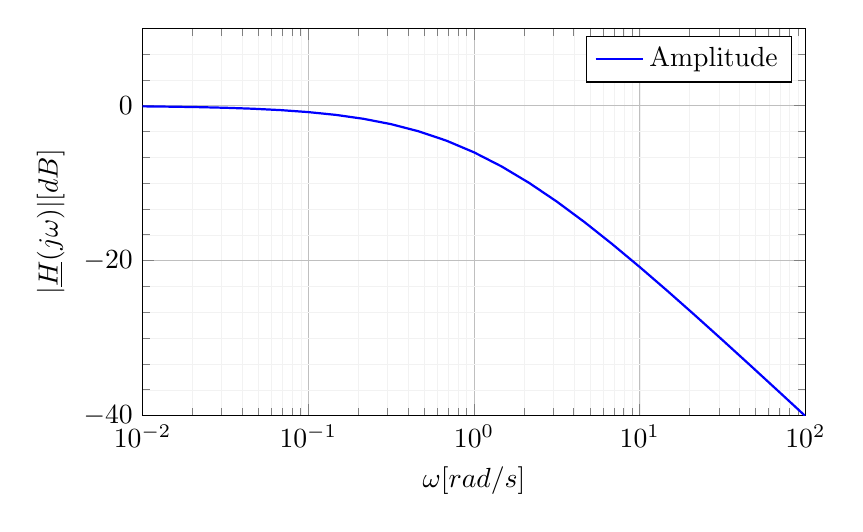
\begin{tikzpicture}
        \begin{semilogxaxis}[
            xlabel={$\omega [rad/s]$},
            ylabel={$|\underline{H}(j\omega)|[dB]$},
            xmin=0.01, xmax=100,
            ymin=-40, ymax=10,
            xmode=log,
            grid=both,
            grid style={line width=.1pt, draw=gray!10},
            major grid style={line width=.2pt,draw=gray!50},
            minor tick num=5,
            width=10cm,
            height=6.5cm,
            ]

            \addplot[domain=0.01:100, blue, thick] {
                20 * log10(1/(1+x))
            };
            \addlegendentry{Amplitude};
        \end{semilogxaxis}
    \end{tikzpicture}
\end{center}
\textbf{Phasengang:}
\begin{center}
    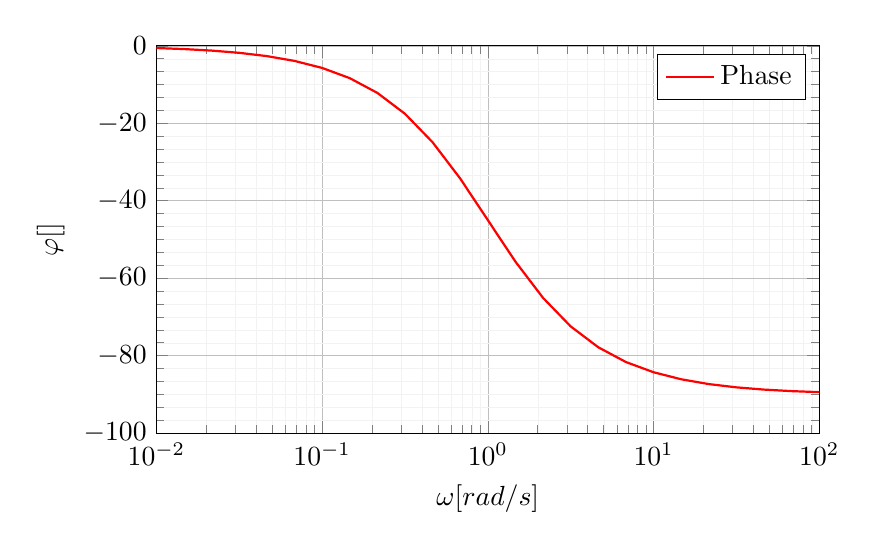
\begin{tikzpicture}
        \begin{semilogxaxis}[
                xlabel={$\omega [rad/s]$},
                ylabel={$\varphi [\degree]$},
                xmin=0.01, xmax=100,
                ymin=-100, ymax=0,
                xmode=log,
                grid=both,
                grid style={line width=.1pt, draw=gray!10},
                major grid style={line width=.2pt,draw=gray!50},
                minor tick num=5,
                width=10cm,
                height=6.5cm,
            ]

            \addplot[domain=0.01:100, red, thick] {-atan(x/1)};
            \addlegendentry{Phase};

        \end{semilogxaxis}
    \end{tikzpicture}
\end{center}
\subsection{Umrechnen rad/s nach Hz}

Die Kreisfrequenz \( \omega \) wird in Einheiten Radiant pro Sekunde (\(
\text{rad/s} \)) angegeben und beschreibt, wie schnell sich ein periodisches
Signal pro Sekunde vollständig umkreist oder vollständig durchläuft. \\ Die
Frequenz \( f \) wird in Hertz (\( \text{Hz} \)) gemessen und gibt an, wie oft
sich ein periodisches Signal innerhalb einer Sekunde wiederholt oder wie viele
vollständige Zyklen es pro Sekunde durchläuft. \\ Die Umrechnung zwischen \(
\omega \) und \( f \) erfolgt durch folgende Formel:

\[
    \omega = 2 \pi f
\]
\\
Umrechnung von \( f \) zu \( \omega \)
\[
    f = \frac{\omega}{2 \pi}
\]

\section{Filter}
\subsection{Grenzfrequnez}
Die Grenzfrequnez bezeichnet die Frequenz, bei der ein Filter anfängt, Signale
zu beeinflussen oder zu verändern.
\begin{itemize}

    \item \textbf{Definition:} Die Grenzfrequenz ist bei 3 dB definiert, an diesem Punkt ist das Ausgangssignal im Vergleich zum Eingangssignal um 3 dB abgeschwächt. 3 dB entspricht $\sqrt{\frac{1}{2}} = \frac{1}{\sqrt{2}} = 0,7071$. Das entspricht 70,71\% der Eingangsspannung.

    \item \textbf{Bandbreite:} Die Bandbreite eines Filters ist zwischen den beiden 3-dB-Punkten definiert.

    \item \textbf{Phase:} Bei Filtern erster Ordnung beträgt die Phasenverschiebung bei der Grenzfrequenz etwa 45 Grad.

\end{itemize}
\newpage
\subsection{Tiefpass}
Ein Tiefpassfilter lässt Signale mit niedrigen Frequenzen passieren, während hohe Frequenzen blockiert werden. Filter 1.Ordnung können
durch LR- oder RC-Glieder aufgebaut werden. \\\\ 
\textbf{RC-Glied}
\begin{center}
    \begin{circuitikz}
        \draw (0,0) to[R=$R$] (2,0);
        \draw (2,0) to[C=$C$] (2,-1.5);
        \draw (0,-1.5) -- (3,-1.5);
        \draw (2,0) -- (3,0);
        \draw[->,blue,>=latex,fill=blue] (0,-0.25) -- (0,-1.25) node[midway, left,blue] {${U}_e$};
        \draw[->,blue,>=latex,fill=blue] (3,-0.25) -- (3,-1.25) node[midway, right,blue] {${U}_a$};
        \draw[black,fill=black] (2,0) circle (1.5pt);
        \draw[black,fill=black] (2,-1.5) circle (1.5pt);
        \draw[black] (0,0) circle (1.5pt);
        \draw[black] (0,-1.5) circle (1.5pt);
        \draw[black] (3,0) circle (1.5pt);
        \draw[black] (3,-1.5) circle (1.5pt);
    \end{circuitikz}
\end{center}
Übertragungsfunktion:

\[ \underline{H}(j\omega) = \frac{\underline{U_{a}}(j\omega)}{\underline{U_{e}}(j\omega)}=\frac{X_{C}}{R+X_{C}}=\frac{\frac{1}{j \omega C}}{R+\frac{1}{j \omega C}}=\frac{1}{1+j\omega R C}=\frac{1}{\sqrt{1+(\omega C R)^2}}\]
\\
Berechnung Grenzfrequenz:

\[ f_{g} = \frac{1}{2\pi RC} \]
\\
\textbf{LR-Glied}
\begin{center}
    \begin{circuitikz}
        \ctikzset{inductors/scale=1, inductor=american}
        \draw (0,0) to[L=$L$] (2,0);
        \draw (2,0) to[R=$R$] (2,-1.5);
        \draw (0,-1.5) -- (3,-1.5);
        \draw (2,0) -- (3,0);
        \draw[->,blue,>=latex,fill=blue] (0,-0.25) -- (0,-1.25) node[midway, left,blue] {${U}_e$};
        \draw[->,blue,>=latex,fill=blue] (3,-0.25) -- (3,-1.25) node[midway, right,blue] {${U}_a$};
        \draw[black,fill=black] (2,0) circle (1.5pt);
        \draw[black,fill=black] (2,-1.5) circle (1.5pt);
        \draw[black] (0,0) circle (1.5pt);
        \draw[black] (0,-1.5) circle (1.5pt);
        \draw[black] (3,0) circle (1.5pt);
        \draw[black] (3,-1.5) circle (1.5pt);
    \end{circuitikz}
\end{center}
Übertragungsfunktion:

\[ \underline{H}(j\omega) = \frac{\underline{U_{a}}(j\omega)}{\underline{U_{e}}(j\omega)}=\frac{R}{X_{L}+R}=\frac{R}{j\omega L+R}=\frac{1}{1+\frac{j\omega L}{R}}=\frac{1}{\sqrt{1+(\frac{\omega L}{R})^2}}\]
\\
Berechnung Grenzfrequenz:

\[ f_{g} = \frac{R}{2\pi L} \]
\\
\textbf{Amplitudengang:}
\begin{center}
    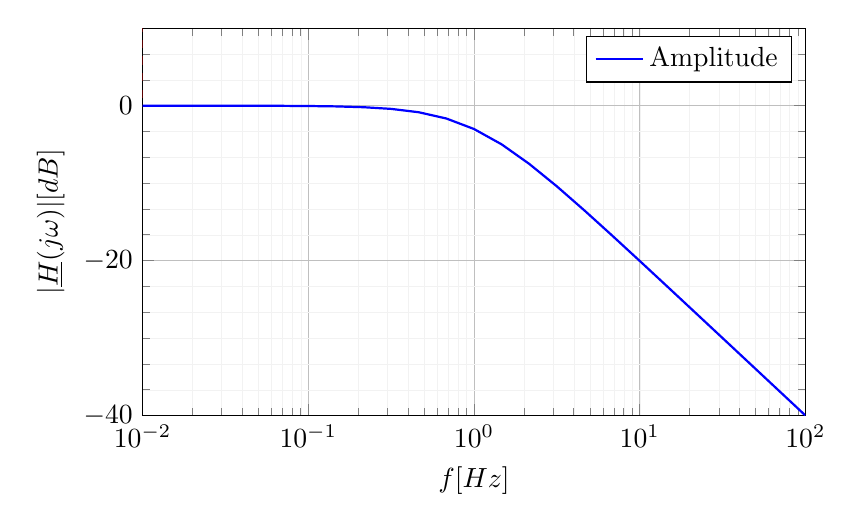
\begin{tikzpicture}
        \begin{semilogxaxis}[
            xlabel={$f [Hz]$},
            ylabel={$|\underline{H}(j\omega)|[dB]$},
            xmin=0.01, xmax=100,
            ymin=-40, ymax=10,
            xmode=log,
            grid=both,
            grid style={line width=.1pt, draw=gray!10},
            major grid style={line width=.2pt,draw=gray!50},
            minor tick num=5,
            width=10cm,
            height=6.5cm,
            ]

            \addplot[domain=0.01:100, blue, thick] {
                20 * log10(1/sqrt(1+(x)^2))
            };
            \draw[dashed, red] (0.01,1) -- (0.01,420) node[red,above] {$f_{\text{g}}$};
            \addlegendentry{Amplitude};
        \end{semilogxaxis}
    \end{tikzpicture}
\end{center}
\textbf{Phasengang:}
\begin{center}
    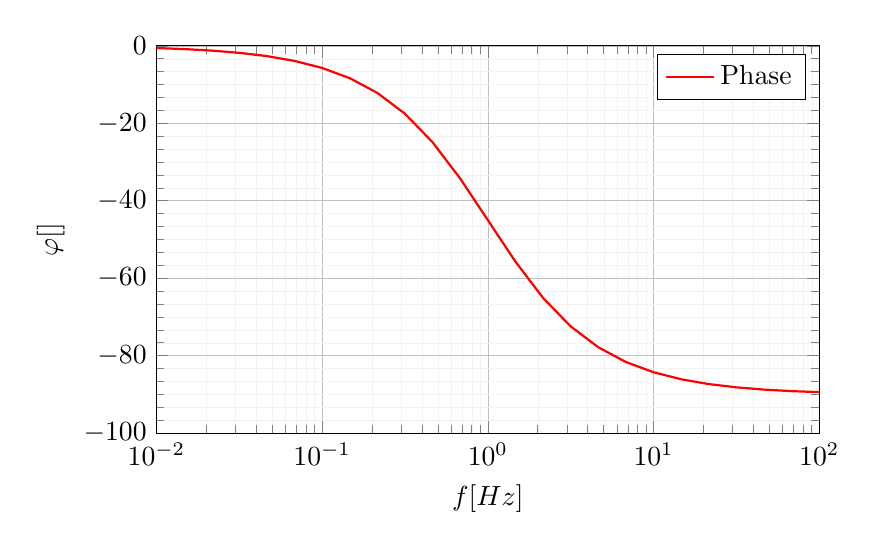
\begin{tikzpicture}
        \begin{semilogxaxis}[
                xlabel={$f [Hz]$},
                ylabel={$\varphi [\degree]$},
                xmin=0.01, xmax=100,
                ymin=-100, ymax=0,
                xmode=log,
                grid=both,
                grid style={line width=.1pt, draw=gray!10},
                major grid style={line width=.2pt,draw=gray!50},
                minor tick num=5,
                width=10cm,
                height=6.5cm,
            ]

            \addplot[domain=0.01:100, red, thick] {-atan(x/1)};
            \draw[dashed, red] (0.01,1) -- (0.01,80) node[red,above] {$f_{\text{g}}$};

            \addlegendentry{Phase};

        \end{semilogxaxis}
    \end{tikzpicture}
\end{center}
\newpage
\subsection{Hochpass}
Ein Hochpassfilter lässt nur Signale mit hohen Frequenzen passieren und blockiert niedrige Frequenzen. Filter erster Ordnung können mit RC- oder RL-Gliedern realisiert werden.
\textbf{RC-Glied}
\begin{center}
    \begin{circuitikz}
        \draw (2,0) to[R=$R$] (2,-1.5);
        \draw (0,0) to[C=$C$] (2,0);
        \draw (0,-1.5) -- (3,-1.5);
        \draw (2,0) -- (3,0);
        \draw[->,blue,>=latex,fill=blue] (0,-0.25) -- (0,-1.25) node[midway, left,blue] {$U_{\text{e}}$};
        \draw[->,blue,>=latex,fill=blue] (3,-0.25) -- (3,-1.25) node[midway, right,blue] {$U_{\text{a}}$};
        \draw[black,fill=black] (2,0) circle (1.5pt);
        \draw[black,fill=black] (2,-1.5) circle (1.5pt);
        \draw[black] (0,0) circle (1.5pt);
        \draw[black] (0,-1.5) circle (1.5pt);
        \draw[black] (3,0) circle (1.5pt);
        \draw[black] (3,-1.5) circle (1.5pt);
    \end{circuitikz}
\end{center}
Übertragungsfunktion:

\[ \underline{H}(j\omega) = \frac{\underline{U_{a}}(j\omega)}{\underline{U_{e}}(j\omega)}=\frac{R}{X_{C}+R}=\frac{R}{\frac{1}{j \omega C}+R}=\frac{1}{1+\frac{1}{j\omega R C}}=\frac{1}{\sqrt{1+\frac{1}{(\omega R C)^2}}}\]
\\
Berechnung Grenzfrequenz:

\[ f_{g} = \frac{1}{2\pi RC} \]
\\
\textbf{RL-Glied}
\begin{center}
    \begin{circuitikz}
        \ctikzset{inductors/scale=1, inductor=american}
        \draw (0,0) to[R=$R$] (2,0);
        \draw (2,0) to[L=$L$] (2,-1.5);
        \draw (0,-1.5) -- (3,-1.5);
        \draw (2,0) -- (3,0);
        \draw[->,blue,>=latex,fill=blue] (0,-0.25) -- (0,-1.25) node[midway, left,blue] {${U}_e$};
        \draw[->,blue,>=latex,fill=blue] (3,-0.25) -- (3,-1.25) node[midway, right,blue] {${U}_a$};
        \draw[black,fill=black] (2,0) circle (1.5pt);
        \draw[black,fill=black] (2,-1.5) circle (1.5pt);
        \draw[black] (0,0) circle (1.5pt);
        \draw[black] (0,-1.5) circle (1.5pt);
        \draw[black] (3,0) circle (1.5pt);
        \draw[black] (3,-1.5) circle (1.5pt);
    \end{circuitikz}
\end{center}
Übertragungsfunktion:

\[ \underline{H}(j\omega) = \frac{\underline{U_{a}}(j\omega)}{\underline{U_{e}}(j\omega)}=\frac{X_{L}}{R+X_{L}}=\frac{j \omega L}{R+j \omega L}=\frac{1}{1+\frac{R}{j\omega L}}=\frac{1}{\sqrt{1+(\frac{R}{\omega L})^2}}\]
\\
Berechnung Grenzfrequenz:

\[ f_{g} = \frac{R}{2\pi L} \]
\\
\textbf{Amplitudengang:}
\begin{center}
    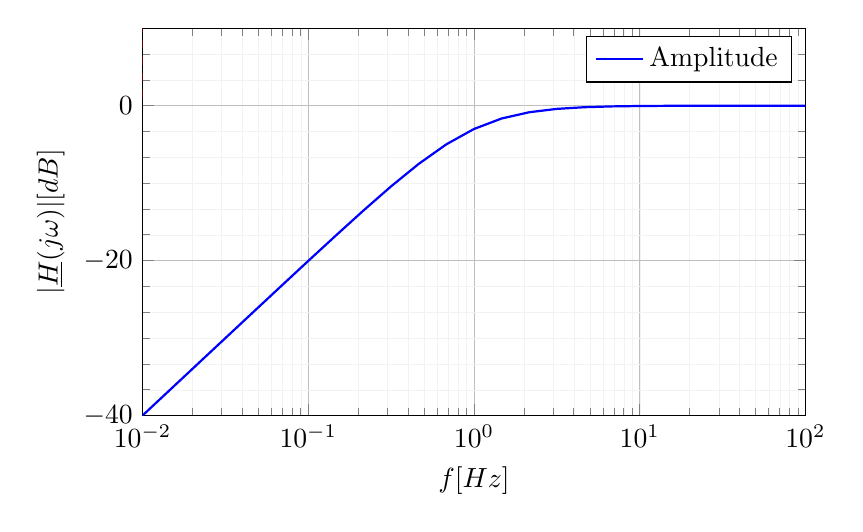
\begin{tikzpicture}
        \begin{semilogxaxis}[
            xlabel={$f [Hz]$},
            ylabel={$|\underline{H}(j\omega)|[dB]$},
            xmin=0.01, xmax=100,
            ymin=-40, ymax=10,
            xmode=log,
            grid=both,
            grid style={line width=.1pt, draw=gray!10},
            major grid style={line width=.2pt,draw=gray!50},
            minor tick num=5,
            width=10cm,
            height=6.5cm,
            ]

            \addplot[domain=0.01:100, blue, thick] {
                20 * log10(1/sqrt(1+(1/x)^2))
            };
            \draw[dashed, red] (0.01,1) -- (0.01,420) node[red,above] {$f_{\text{g}}$};
            \addlegendentry{Amplitude};
        \end{semilogxaxis}
    \end{tikzpicture}
\end{center}
\textbf{Phasengang:}
\begin{center}
    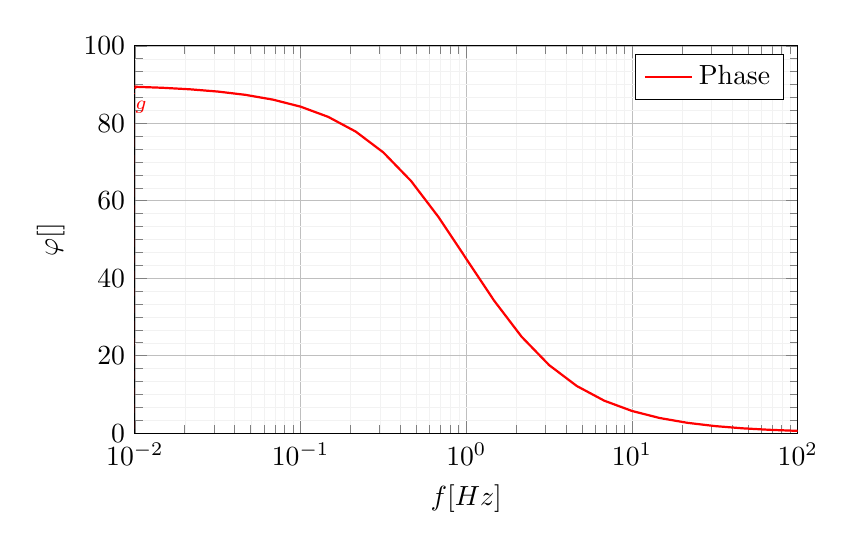
\begin{tikzpicture}
        \begin{semilogxaxis}[
                xlabel={$f [Hz]$},
                ylabel={$\varphi [\degree]$},
                xmin=0.01, xmax=100,
                ymin=0, ymax=100,
                xmode=log,
                grid=both,
                grid style={line width=.1pt, draw=gray!10},
                major grid style={line width=.2pt,draw=gray!50},
                minor tick num=5,
                width=10cm,
                height=6.5cm,
            ]
            \addplot[domain=0.01:100, red, thick] {atan(1/x)};
            \draw[dashed, red] (0.01,1) -- (0.01,80) node[red,above] {$f_{\text{g}}$};
            \addlegendentry{Phase};

        \end{semilogxaxis}
    \end{tikzpicture}
\end{center}

\subsection{Bandpass !TODO!}
Ein Bandpassfilter lässt nur Signale innerhalb eines bestimmten
Frequenzbereichs passieren und blockiert Signale außerhalb dieses Bereichs.
Filter 1.Ordnung können durch RC-Netzwerk aufgebaut werden.\\\\
\textbf{RC-Netzwerk}
\begin{center}
    \begin{circuitikz}
        \draw (2.25,0) to[C=$C$] (2.25,-1.5);
        \draw (0,0) to[R=$R$] (2.25,0);
        \draw (2.25,0) to[C=$C$] (4,0);
        \draw (4,0) to[R=$R$] (4,-1.5);
        \draw (4,0) -- (5,0);
        \draw (0,-1.5) -- (5,-1.5);
        \draw[->,blue,>=latex,fill=blue] (0,-0.25) -- (0,-1.25) node[midway, left,blue] {$U_{\text{e}}$};
        \draw[->,blue,>=latex,fill=blue] (5,-0.25) -- (5,-1.25) node[midway, right,blue] {$U_{\text{a}}$};
        \draw[black,fill=black] (2.25,0) circle (1.5pt);
        \draw[black,fill=black] (2.25,-1.5) circle (1.5pt);
        \draw[black,fill=black] (4,0) circle (1.5pt);
        \draw[black,fill=black] (4,-1.5) circle (1.5pt);
        \draw[black] (0,0) circle (1.5pt);
        \draw[black] (0,-1.5) circle (1.5pt);
        \draw[black] (5,0) circle (1.5pt);
        \draw[black] (5,-1.5) circle (1.5pt);
    \end{circuitikz}
\end{center}

Übertragungsfunktion:
\[ \underline{H}(j\omega) = \frac{\underline{U_{a}}(j\omega)}{\underline{U_{e}}(j\omega)}= \frac{1}{3+j(\omega R C-\frac{1}{\omega *R *C})}=\frac{1}{\sqrt{9+(\omega RC-\frac{1}{\omega RC})^2}}\]
\\
Berechnung Grenzfrequenzen:

\[ f_{0} = \frac{1}{2\pi RC} \]
\[ f_{0} = \sqrt{f_{oben}*f_{unten}} \]
\[ B= f_{oben}-f_{unten} \]

\textbf{Amplitudengang:}
\begin{center}
    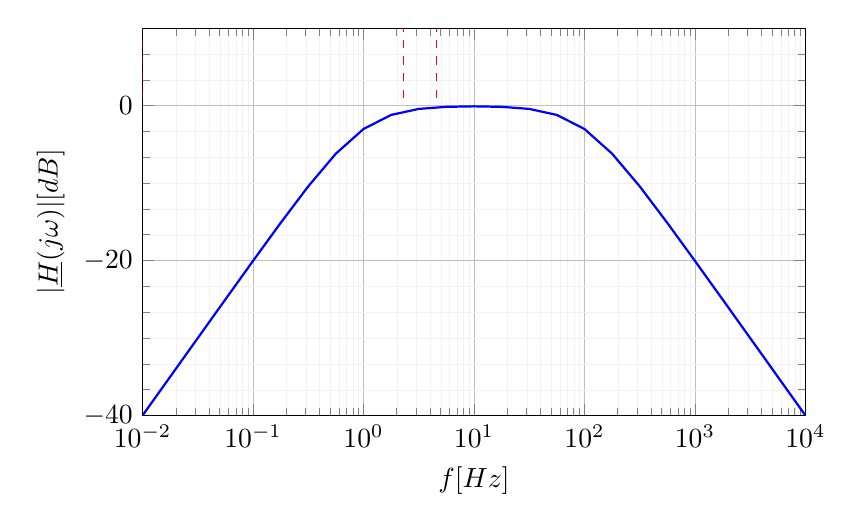
\begin{tikzpicture}
        \begin{semilogxaxis}[
            xlabel={$f [Hz]$},
            ylabel={$|\underline{H}(j\omega)|[dB]$},
            xmin=0.01, xmax=10000,
            ymin=-40, ymax=10,
            xmode=log,
            grid=both,
            grid style={line width=.1pt, draw=gray!10},
            major grid style={line width=.2pt,draw=gray!50},
            minor tick num=5,
            width=10cm,
            height=6.5cm,
            ]

            \addplot[domain=0.01:10000, blue, thick] {
                20*log10((x/sqrt(1+x^2)) / sqrt(1+(x/100)^2))
                %20*log10(1/(sqrt(9+(x*0.1-(1/(x*0.1)))^2)))
            };
            %\addlegendentry{Amplitude};

            \draw[dashed, red] (0.01,1) -- (0.01,420) node[red,above] {$f_{\text{unten}}$};
            \draw[dashed, red] (4.6,1) -- (4.6, 420) node[above, red] {$f_{\text{oben}}$};
            \draw[dashed, red] (2.3,1) -- (2.3,420) node[red,above] {$f_{\text{0}}$};

        \end{semilogxaxis}
    \end{tikzpicture}
\end{center}
\textbf{Phasengang:}
\begin{center}
    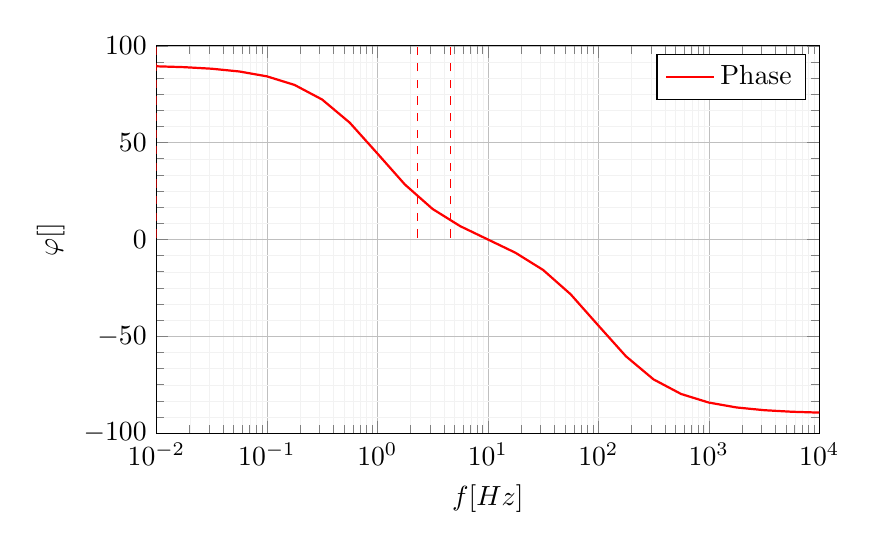
\begin{tikzpicture}
        \begin{semilogxaxis}[
                xlabel={$f [Hz]$},
                ylabel={$\varphi [\degree]$},
                xmin=0.01, xmax=10000,
                ymin=-100, ymax=100,
                xmode=log,
                grid=both,
                grid style={line width=.1pt, draw=gray!10},
                major grid style={line width=.2pt,draw=gray!50},
                minor tick num=5,
                width=10cm,
                height=6.5cm,
            ]
            \addplot[domain=0.01:10000, red, thick] {
                atan(1/x)-atan(x/100)
                %-atan((1/3)*(x*0.1-(1/(x*0.1))))
            };

            \draw[dashed, red] (0.01,1) -- (0.01,170) node[red,above] {$f_{\text{unten}}$};
            \draw[dashed, red] (4.6,1) -- (4.6, 170) node[above, red] {$f_{\text{oben}}$};
            \draw[dashed, red] (2.3,1) -- (2.3,170) node[red,above] {$f_{\text{0}}$};

            \addlegendentry{Phase};

        \end{semilogxaxis}
    \end{tikzpicture}
\end{center}

\subsection{Allpass}
Ein Allpassfilter lässt alle Frequenzen passieren, ändert jedoch die Phasenlage der Signale, während die Amplituden unverändert bleiben.

\textbf{Amplitudengang:}
\begin{center}
    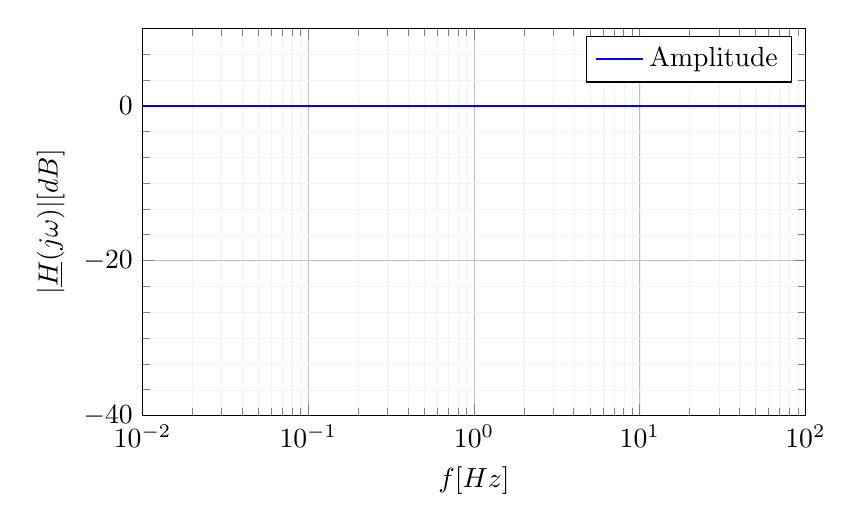
\begin{tikzpicture}
        \begin{semilogxaxis}[
            xlabel={$f [Hz]$},
            ylabel={$|\underline{H}(j\omega)|[dB]$},
            xmin=0.01, xmax=100,
            ymin=-40, ymax=10,
            xmode=log,
            grid=both,
            grid style={line width=.1pt, draw=gray!10},
            major grid style={line width=.2pt,draw=gray!50},
            minor tick num=5,
            width=10cm,
            height=6.5cm,
            ]

            \addplot[domain=0.01:100, blue, thick] {
                20 * log10(1)
            };
            \addlegendentry{Amplitude};
        \end{semilogxaxis}
    \end{tikzpicture}
\end{center}
\textbf{Phasengang:}
\begin{center}
    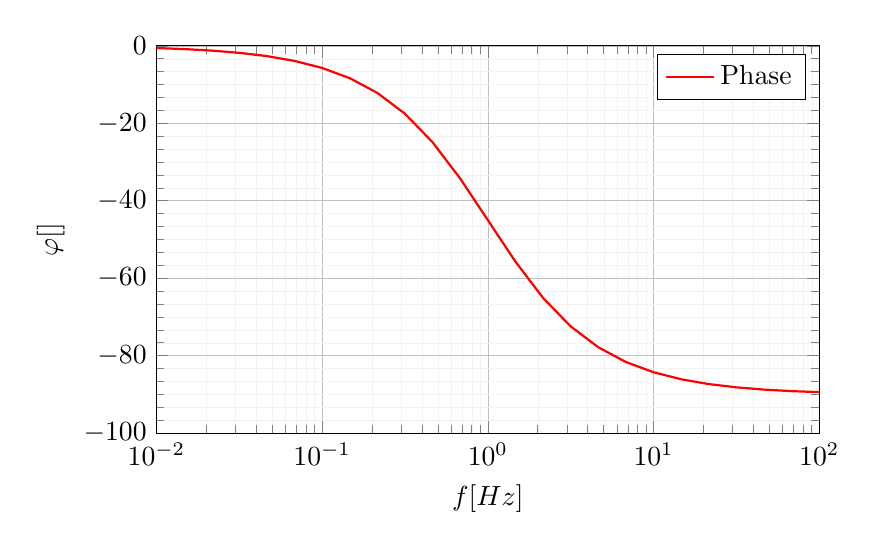
\begin{tikzpicture}
        \begin{semilogxaxis}[
                xlabel={$f [Hz]$},
                ylabel={$\varphi [\degree]$},
                xmin=0.01, xmax=100,
                ymin=-100, ymax=0,
                xmode=log,
                grid=both,
                grid style={line width=.1pt, draw=gray!10},
                major grid style={line width=.2pt,draw=gray!50},
                minor tick num=5,
                width=10cm,
                height=6.5cm,
            ]
            \addplot[domain=0.01:100, red, thick] {-atan(x)};
            \addlegendentry{Phase};

        \end{semilogxaxis}
    \end{tikzpicture}
\end{center}